\documentclass[12pt,a4paper]{article}

% ─── Page Layout ───────────────────────────────────────────────────────────────
\usepackage[a4paper, margin=0.8in, headheight=14pt]{geometry}

% ─── Fonts (XeLaTeX) ───────────────────────────────────────────────────────────
\usepackage{fontspec}
\usepackage{unicode-math}
\setmainfont{TeX Gyre Pagella}
\setmonofont[Scale=0.88]{TeX Gyre Cursor}
\setmathfont{Latin Modern Math}

% ─── Packages ──────────────────────────────────────────────────────────────────
\usepackage{xcolor}
\usepackage{colortbl}
\usepackage{titlesec}
\usepackage{enumitem}
\usepackage{tabularx}
\usepackage{booktabs}
\usepackage{array}
\usepackage{amsmath}
\usepackage{tikz}
\usetikzlibrary{shapes.geometric, arrows.meta, positioning, calc, fit, decorations.pathreplacing}
\usepackage{tcolorbox}
\tcbuselibrary{skins, breakable}
\usepackage{hyperref}
\usepackage{fancyhdr}
\usepackage{graphicx}
\usepackage{microtype}
\hyphenpenalty=10000
\exhyphenpenalty=10000
\sloppy
\usepackage{caption}
\usepackage{setspace}
\usepackage{multirow}
\usepackage{tocloft}

% ─── Q&A helper ────────────────────────────────────────────────────────────────
\newcommand{\Q}[1]{\textbf{#1}\par\noindent\ignorespaces}

% ─── Colour Palette ────────────────────────────────────────────────────────────
\definecolor{myred}{RGB}{196,30,58}
\definecolor{mydark}{RGB}{30,30,50}
\definecolor{mygreen}{RGB}{14,120,80}
\definecolor{myteal}{RGB}{0,130,140}
\definecolor{myamber}{RGB}{180,100,0}
\definecolor{mypurple}{RGB}{100,30,160}
\definecolor{mygray}{RGB}{246,247,249}
\definecolor{mgframe}{RGB}{180,185,200}
\definecolor{watermark}{RGB}{145,150,170}
\definecolor{hdrred}{RGB}{250,232,235}
\definecolor{hdrgreen}{RGB}{220,244,233}
\definecolor{hdrteal}{RGB}{220,242,244}
\definecolor{hdramber}{RGB}{253,242,215}
\definecolor{hdrpurple}{RGB}{238,228,255}
\definecolor{hdrgray}{RGB}{238,240,245}
\definecolor{rowalt}{RGB}{250,251,253}

% ─── Section Formatting ────────────────────────────────────────────────────────
\titleformat{\section}
  {\large\bfseries\color{myred}}{\thesection.}{0.5em}{}
  [\vspace{1pt}{\color{myred}\rule{\linewidth}{0.8pt}}]
\titleformat{\subsection}
  {\normalsize\bfseries\color{myteal}}{\thesubsection}{0.5em}{}
\titlespacing*{\section}{0pt}{18pt}{7pt}
\titlespacing*{\subsection}{0pt}{11pt}{4pt}

% ─── Paragraph ─────────────────────────────────────────────────────────────────
\setlength{\parindent}{0pt}
\setlength{\parskip}{4pt}

% ─── TOC Styling ───────────────────────────────────────────────────────────────
\renewcommand{\cfttoctitlefont}{\large\bfseries\color{myred}}
\renewcommand{\cftaftertoctitle}{\par\noindent{\color{myred}\rule{\linewidth}{0.8pt}}}
\setlength{\cftbeforetoctitleskip}{0pt}
\setlength{\cftaftertoctitleskip}{6pt}
\renewcommand{\cftsecfont}{\normalsize\bfseries\color{mydark}}
\renewcommand{\cftsecpagefont}{\normalsize\bfseries\color{mydark}}
\renewcommand{\cftsecleader}{\cftdotfill{\cftdotsep}}
\setlength{\cftbeforesecskip}{7pt}
\renewcommand{\cftsubsecfont}{\small\color{mydark}}
\renewcommand{\cftsubsecpagefont}{\small\color{mydark}}
\setlength{\cftbeforesubsecskip}{3pt}
\setlength{\cftsubsecindent}{1.4em}

% ─── Table helpers ─────────────────────────────────────────────────────────────
\renewcommand{\arraystretch}{1.45}
\setlength{\tabcolsep}{6pt}
\arrayrulecolor{mydark}
\newcolumntype{B}[1]{>{\small\bfseries\raggedright\arraybackslash}m{#1}}
\newcolumntype{Y}{>{\small\raggedright\arraybackslash}X}
\renewcommand{\tabularxcolumn}[1]{m{#1}}

% ─── Header / Footer ───────────────────────────────────────────────────────────
\pagestyle{fancy}
\fancyhf{}
\fancyhead[L]{\small\color{myred}\textbf{EC502}\;\color{mydark}--- Computer Architecture}
\fancyhead[R]{\small\color{myteal}\textbf{Module 1 Notes}}
\fancyfoot[C]{\small\color{mydark}\thepage}
\fancyfoot[R]{\small\color{watermark}\textit{\copyright\ Biraj}}
\renewcommand{\headrulewidth}{0.5pt}
\renewcommand{\footrulewidth}{0.3pt}

% ─── Hyperref ──────────────────────────────────────────────────────────────────
\hypersetup{
  colorlinks=true, linkcolor=myteal, urlcolor=myteal,
  pdfauthor={Biraj Sarkar},
  pdftitle={EC502 --- Module 1 Notes}
}

% ─── tcolorbox styles ──────────────────────────────────────────────────────────
\tcbset{
  tikzbox/.style={
    colback=mygray, colframe=mgframe, boxrule=0.6pt, arc=4pt,
    left=8pt, right=8pt, top=6pt, bottom=6pt,
    colbacktitle=mgframe, coltitle=mydark,
    fonttitle=\small\bfseries
  },
  defbox/.style={
    colback=hdrgreen, colframe=mygreen, boxrule=0.8pt, arc=4pt,
    left=9pt, right=9pt, top=6pt, bottom=6pt,
    colbacktitle=mygreen, coltitle=white,
    fonttitle=\small\bfseries
  },
  formulabox/.style={
    colback=hdrteal, colframe=myteal, boxrule=0.8pt, arc=4pt,
    left=9pt, right=9pt, top=7pt, bottom=7pt,
    colbacktitle=myteal, coltitle=white,
    fonttitle=\small\bfseries
  },
  examplebox/.style={
    colback=hdramber, colframe=myamber, boxrule=0.8pt, arc=4pt,
    left=9pt, right=9pt, top=6pt, bottom=6pt,
    colbacktitle=myamber, coltitle=white,
    fonttitle=\small\bfseries
  },
  masonbox/.style={
    colback=hdrpurple, colframe=mypurple, boxrule=0.8pt, arc=4pt,
    left=9pt, right=9pt, top=6pt, bottom=6pt,
    colbacktitle=mypurple, coltitle=white,
    fonttitle=\small\bfseries
  },
  exambox/.style={
    colback=hdrpurple, colframe=mypurple, boxrule=1pt, arc=5pt,
    left=10pt, right=10pt, top=8pt, bottom=8pt,
    colbacktitle=mypurple, coltitle=white,
    fonttitle=\bfseries,
    breakable, title after break={\textbf{Frequently Asked / Viva Questions (contd.)}}}
}
% Make all boxes breakable across pages
\tcbset{breakable}

% ─── TikZ styles ───────────────────────────────────────────────────────────────
\tikzset{
  block/.style={rectangle, draw=myteal, fill=hdrteal,
    text width=2.4cm, align=center, minimum height=0.95cm,
    font=\small, rounded corners=3pt, line width=0.7pt},
  redblock/.style={rectangle, draw=myred, fill=hdrred,
    text width=2.4cm, align=center, minimum height=0.95cm,
    font=\small, rounded corners=3pt, line width=0.7pt},
  netnode/.style={rectangle, draw=myteal, fill=hdrteal,
    text width=1.5cm, align=center, minimum height=0.8cm,
    font=\small, rounded corners=3pt, line width=0.7pt},
  sumjunc/.style={circle, draw=myamber, fill=hdramber,
    minimum size=0.62cm, font=\small, line width=0.8pt},
  snode/.style={circle, draw=mypurple, fill=hdrpurple,
    minimum size=0.55cm, font=\footnotesize, line width=0.7pt},
  arrow/.style={-Stealth, thick, color=mydark},
  redarrow/.style={-Stealth, thick, color=myred},
  line/.style={thick, color=mydark}
}

% ═══════════════════════════════════════════════════════════════════════════════
\begin{document}
% ═══════════════════════════════════════════════════════════════════════════════

\begin{center}
  {\LARGE\bfseries\color{myred} EC502 --- Computer Architecture}\\[5pt]
  {\normalsize\color{mydark} Semester V \quad$\bullet$\quad 3L:0T:0P \quad$\bullet$\quad 3 Credits}\\[3pt]
  {\normalsize\color{myteal}\textbf{Module 1 Exam Notes: Computer Structure and Instruction Sets}}\\[3pt]
  {\small\color{mydark} CGEC \;$|$\; B.Tech ECE (2023--27) \;$|$\; \textit{Biraj Sarkar}}
\end{center}
\vspace{2pt}
\noindent{\color{myred}\rule{\linewidth}{1.5pt}}
\vspace{2pt}

\hypersetup{linkcolor=mydark}
\tableofcontents
\hypersetup{linkcolor=myteal}
\newpage

\section{Computer Structure and Instruction Sets}
\begin{tcolorbox}[defbox,title={Architecture and organisation}]
Computer architecture specifies the features visible to software, including instructions, registers, data types and addressing rules. Organisation describes the hardware arrangement that implements those features, such as datapaths, buses, caches and control.
\end{tcolorbox}
\subsection{Functional units and stored programs}
\begin{itemize}[leftmargin=*,itemsep=3pt]
\item \textbf{Input and output.} Device controllers accept inputs and deliver outputs. They expose data, status and control registers to the processor and transfer data to or from memory as required.
\item \textbf{Main memory.} Holds instructions and data at addressable locations. In a byte-addressed machine each address selects one byte. A word typically occupies several successive bytes.
\item \textbf{Central processing unit (CPU).} Registers hold operands and instruction state. The arithmetic logic unit (ALU) operates on data. The control unit selects data paths and sequences operations.
\item \textbf{System interconnection.} Address signals identify a location or device. Data signals convey the value. Control signals specify read, write, request, acknowledgement and similar events.
\item \textbf{Stored-program principle.} Instruction bit patterns reside in memory. A Von Neumann organisation shares a path for instructions and data, so traffic can contend for that path. Harvard organisation separates instruction and data paths. Split instruction/data caches can feed a processor that uses a unified main memory.
\end{itemize}
\begin{tcolorbox}[tikzbox,title={Functional units and their interconnection},unbreakable]
\centering
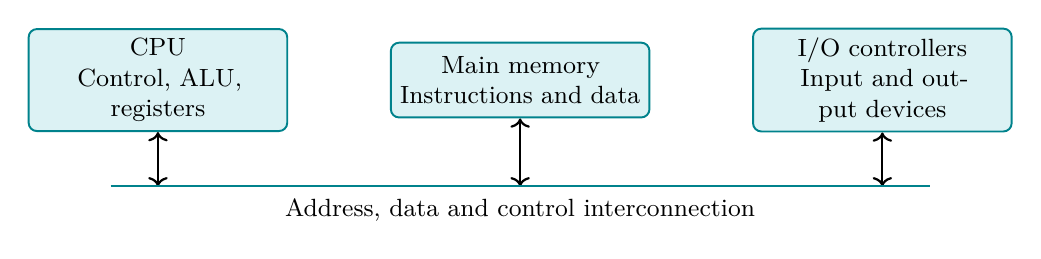
\begin{tikzpicture}[font=\small]
\node[block,text width=3.05cm] (cpu) at (0,0) {CPU\\Control, ALU, registers};
\node[block,text width=3.05cm] (mem) at (4.6,0) {Main memory\\Instructions and data};
\node[block,text width=3.05cm] (io) at (9.2,0) {I/O controllers\\Input and output devices};
\draw[<->,thick] (cpu.south)--(0,-1.35);
\draw[<->,thick] (mem.south)--(4.6,-1.35);
\draw[<->,thick] (io.south)--(9.2,-1.35);
\draw[thick,myteal] (-.6,-1.35)--(9.8,-1.35);
\node[below] at (4.6,-1.38) {Address, data and control interconnection};
\end{tikzpicture}
\end{tcolorbox}

\subsection{Software and program translation}
\begin{itemize}[leftmargin=*,itemsep=3pt]
\item \textbf{Application software} performs a user task. \textbf{System software} includes the operating system, device drivers and language tools. The operating system manages processor time, memory, files and devices.
\item \textbf{Compiler and assembler.} A compiler generally translates high-level source to assembly or object code. An assembler translates mnemonics to machine encodings, resolves local labels and records unresolved addresses for relocation.
\item \textbf{Linker and loader.} A linker combines object files and libraries, resolves symbols and relocates references. A loader maps a program into memory and transfers control to its entry point.
\item \textbf{Performance impact.} Algorithm and compiler change executed instruction count and locality. The operating system can add scheduling, interrupt and I/O time. Compare actual workloads and execution time.
\end{itemize}
\subsection{Execution time, CPI and Amdahl's law}
\begin{tcolorbox}[defbox,title={Latency, throughput and CPI}]
Latency is time for one task. Throughput is work completed per unit time. Cycles per instruction (CPI) is the average number of processor cycles per executed instruction for a workload.
\end{tcolorbox}

For dynamic instruction counts $N_i$ by class, $N=\sum_i N_i$. Count each class's cycles and divide CPU cycles by the clock frequency $f$:
\[
\begin{aligned}
\mathrm{CPI}_{\rm avg}&=\sum_i(N_i/N)\mathrm{CPI}_i,\\
T_{\rm CPU}&=\frac{\sum_i N_i\,\mathrm{CPI}_i}{f}
            =N\,\mathrm{CPI}_{\rm avg}T_{\rm clk},\qquad T_{\rm clk}=1/f .
\end{aligned}
\]
\begin{tcolorbox}[examplebox,title={Compare two implementations on one workload}]
The program executes $60$ million instructions at 1 cycle, $30$ million at 2 cycles, and $10$ million at 5 cycles on machine A.
\[
\begin{aligned}
N&=100\times10^6,\quad
N_{\rm cycles}=(60+60+50)\times10^6,\\
\mathrm{CPI}_A&=1.70,\quad T_A=170\times10^6/(2\times10^9)=85\,\mathrm{ms}.
\end{aligned}
\]
Machine B executes $85$ million instructions at mean CPI 2.4 and $2.4\,\mathrm{GHz}$. $T_B=85\,\mathrm{ms}$ as well. Frequency alone does not determine speed.
\end{tcolorbox}
\begin{itemize}[leftmargin=*,itemsep=3pt]
\item \textbf{Speedup.} Use $T_{\rm old}/T_{\rm new}$ for the same task. Millions of instructions per second (MIPS) equals $f/(10^6\mathrm{CPI})$ when $f$ is in hertz. MIPS can be misleading across instruction sets because each instruction may do a different amount of work.
\item \textbf{Amdahl's law.} If fraction $p$ of the original time runs $s$ times faster, $T_{\rm new}=T_{\rm old}[(1-p)+p/s]$. Overall speedup is $1/[(1-p)+p/s]$. For $p=0.4$ and $s=4$, total speedup is $1/0.7=1.43$, limited to $1/0.6=1.67$ even with unlimited acceleration of that part.
\end{itemize}

\section{Instructions, Addressing and Assembly}
\begin{tcolorbox}[defbox,title={Instruction set architecture}]
An instruction set architecture (ISA) is the hardware--software contract for machine instructions. The opcode identifies the operation. Operand fields identify registers, immediate values or how to locate memory operands.
\end{tcolorbox}
\subsection{Instruction types, formats and instruction cycle}
\begin{itemize}[leftmargin=*,itemsep=3pt]
\item \textbf{Data movement.} Load reads memory to a register. Store writes a register value to memory. Move copies a value, generally without arithmetic.
\item \textbf{Data processing.} Arithmetic, logic, shifts, comparison and bit testing work on operands and may update condition codes.
\item \textbf{Control transfer.} Branch, jump, call and return can replace the sequential next program counter (PC). Conditional branches test a flag or register condition.
\item \textbf{System operations.} System calls, interrupt-return and control-register operations connect application execution with privileged system services.
\end{itemize}
\begin{enumerate}[leftmargin=*,itemsep=3pt]
\item \textbf{Fetch.} Read the instruction addressed by the PC. Compute the sequential successor address (PC plus instruction length).
\item \textbf{Decode.} Interpret the opcode and operand fields. Read registers and form an effective address if required.
\item \textbf{Execute and access memory.} The ALU computes a result, condition or address. An instruction may then read or write data memory.
\item \textbf{Commit architectural effects.} Write destination registers or flags and select the next PC. A branch can override the sequential address.
\end{enumerate}
\par\vspace{6pt}\noindent
\begin{tabularx}{\linewidth}{|B{2.35cm}|Y|Y|}\hline
Format & Example for $X=(A+B)C$ & Where operands are found \\ \hline
Three address & \texttt{ADD T,A,B} then \texttt{MUL X,T,C} & Two explicit inputs and a separate destination. \\ \hline
Two address & \texttt{MOV X,A}, \texttt{ADD X,B}, \texttt{MUL X,C} & One explicit operand is also destination. \\ \hline
One address & \texttt{LOAD A}, \texttt{ADD B}, \texttt{MUL C}, \texttt{STORE X} & Accumulator is implicit. \\ \hline
Zero address & \texttt{PUSH A}, \texttt{PUSH B}, \texttt{ADD}, \texttt{PUSH C}, \texttt{MUL}, \texttt{POP X} & Arithmetic uses the operand stack implicitly. The push/pop instructions can still name addresses. \\ \hline
\end{tabularx}

\begin{tcolorbox}[examplebox,title={Read a toy instruction code}]
Assume a 16-bit format $[\text{opcode:4}][R_d:4][R_s:4][R_t:4]$. If opcode 2 means register addition, hex \texttt{2345} decodes as \texttt{ADD R3,R4,R5}. It writes $R_4+R_5$ into $R_3$. Four opcode bits permit up to 16 primary codes in this format. A different format may use some remaining bits for an immediate or function code.
\end{tcolorbox}
\textbf{ISA styles.} An accumulator ISA uses an implicit accumulator. A stack ISA operates on top-of-stack operands. A general-register ISA may allow register--memory arithmetic or require a load/store model.
\par\vspace{6pt}\noindent
\begin{tabularx}{\linewidth}{|B{2.6cm}|Y|Y|}\hline
Feature & Reduced Instruction Set Computer (RISC) & Complex Instruction Set Computer (CISC) \\ \hline
Encoding & Often uses a small family of regular formats. & Often provides more varied formats and lengths. \\ \hline
Memory operands & Usually explicit loads and stores. Arithmetic operates on registers. & Some arithmetic instructions can directly name a memory operand. \\ \hline
Design effect & Regular operands and encoding can simplify decode and pipelining. & Denser or richer instructions may reduce instruction count, while decode and implementation may need more work. \\ \hline
\end{tabularx}

These are typical design tendencies. Compare CPU time on the same workload because instruction count and implementation both matter.

\subsection{Addressing modes}
Effective address (EA) is the computed memory address of an operand. Let $M[A]$ stand for the contents at address $A$. Assume $R_2=1000$, $R_3=20$, $M[1200]=4000$ and next PC $=2000$.
\par\vspace{6pt}\noindent
\begin{tabularx}{\linewidth}{|B{3.0cm}|Y|Y|}\hline
Mode & Operand or EA rule & Worked reading \\ \hline
Immediate & Literal in instruction & \texttt{\#12} denotes value 12. \\ \hline
Register & Register contents & \texttt{R2} denotes 1000. \\ \hline
Direct & EA is the address field & \texttt{[1200]} reads $M[1200]=4000$. \\ \hline
Memory indirect & EA is the pointer at the address field & Use $M[1200]=4000$ as EA, then read $M[4000]$. \\ \hline
Register indirect & EA is register contents & \texttt{[R2]} reads $M[1000]$. \\ \hline
Base plus displacement & EA is base plus signed constant & \texttt{[R2+16]} has EA $1016$. \\ \hline
Indexed & EA is base plus index, optionally scaled & \texttt{[R2+4*R3]} has EA $1080$. \\ \hline
PC-relative & Branch target is specified PC plus displacement in the chosen units & If relative to next PC and in bytes, $2000-12=1988$. \\ \hline
Auto-increment & Access through a register, then advance it & Word load through $R_2$ with stride 4 uses $1000$ then sets $R_2=1004$. \\ \hline
\end{tabularx}

\subsection{Assembly-language trace}
Assembly instructions typically contain an optional label, mnemonic and operands. A directive guides the assembler, for example to allocate data or place a label. The following illustrative load/store assembly puts the destination operand first.
\begin{tcolorbox}[examplebox,title={Sum three consecutive 32-bit words}]
Start with $R_1=1000$, $R_2=3$, $R_3=0$ and data $7,4,9$ at addresses 1000, 1004, 1008.
\begin{verbatim}
loop: LOAD R4, [R1]
      ADD  R3, R3, R4
      ADDI R1, R1, 4
      SUBI R2, R2, 1
      BNEZ R2, loop
\end{verbatim}
The loaded addresses are 1000, 1004 and 1008. After each iteration $R_3$ is 7, 11 and 20, while $R_2$ is 2, 1 and 0. The branch falls through when the count reaches zero. The address stride is four bytes, not one.
\end{tcolorbox}

\section{Stacks, Queues and Subroutines}
\begin{tcolorbox}[defbox,title={Stack and queue}]
A stack is last-in first-out (LIFO) and supports push/pop at the top. A queue is first-in first-out (FIFO) and inserts at the rear and removes from the front. Stacks support nested calls and expression evaluation. Queues buffer work or data in arrival order.
\end{tcolorbox}

\subsection{Stack convention, calls and returns}
\begin{enumerate}[leftmargin=*,itemsep=2pt]
\item \textbf{Push.} In a full descending stack, subtract word size $w$ from the stack pointer (SP), then write $M[\mathrm{SP}]$. SP points to the top occupied word.
\item \textbf{Pop.} Read $M[\mathrm{SP}]$, then add $w$ to SP. Pushing beyond capacity overflows. Popping an empty stack underflows.
\item \textbf{Call.} Save the next PC in a link register or on the stack, then branch. Save the link before a nested call overwrites it.
\item \textbf{Return.} The calling convention governs arguments, locals and saved registers in the frame. Restore required registers and SP, then load the saved PC.
\end{enumerate}
\begin{tcolorbox}[examplebox,title={Trace a nested call with a downward-growing stack}]
Take $\mathrm{SP}=1000$, $w=4$ and a model that pushes the return address. A call to A saves 104 at 996. A calls B and saves 220 at 992. B returns to 220 and restores $\mathrm{SP}=996$. A returns to 104 and restores $\mathrm{SP}=1000$. Each call unwinds its own frame first.
\end{tcolorbox}
\subsection{Circular hardware queue}
Use $C$ slots with front $h$, next-write position $t$ and occupancy $n$. Enqueue if $n<C$: write at $t$, advance $t$ modulo $C$, and increment $n$. Dequeue if $n>0$: read at $h$, advance $h$ modulo $C$, and decrement $n$. Occupancy distinguishes full from empty when $h=t$. With $C=4$ and both indices at 3, two enqueues use slots 3 and 0.

\newpage
\begin{center}
  {\large\bfseries\color{myred} Quick Revision --- Module 1}\\[3pt]
  {\small\color{mydark} Computer Structure and Instruction Sets $|$ EC502}
\end{center}
\noindent{\color{myred}\rule{\linewidth}{1.2pt}}
\begin{tcolorbox}[formulabox,title={Key Formulas at a Glance}]
\renewcommand{\arraystretch}{1.35}
\begin{tabularx}{\linewidth}{B{5.0cm}Y}
CPU time & $N\cdot\mathrm{CPI}/f$ \\[3pt]
Weighted CPI & $\sum_i(N_i/N)\mathrm{CPI}_i$ \\[3pt]
Amdahl speedup & $1/[(1-p)+p/s]$ \\[3pt]
Scaled index & $\mathrm{EA}=R_b+R_i\cdot\text{scale}+\text{displacement}$ \\[3pt]
Circular index & $\mathrm{next}=(\mathrm{index}+1)\bmod C$ \\[3pt]
\end{tabularx}
\end{tcolorbox}
\begin{tcolorbox}[defbox,title={One-Line Definitions}]
\textbf{Opcode.} Instruction field selecting the operation.\par
\textbf{Effective address.} Address calculated for a memory operand.\par
\textbf{Subroutine.} Callable code that returns control using a saved return address.\par
\end{tcolorbox}
\begin{tcolorbox}[exambox,title={Frequently Asked / Viva Questions}]
\begin{enumerate}[topsep=0pt, label=\textbf{Q\arabic*.}, itemsep=5pt]
\item \Q{What is visible at an ISA boundary?}
Registers, instruction encodings, operations, addressing rules and other programmer-visible state.
\item \Q{Where is the next instruction address held?}
In the program counter.
\item \Q{How do architecture and organisation differ?}
Architecture specifies visible behaviour. Organisation implements it.
\item \Q{What does an assembler produce?}
Encoded machine instructions and, for relocatable objects, symbol and relocation information.
\item \Q{Does a higher clock guarantee lower CPU time?}
Compare instruction count, CPI and frequency together.
\item \Q{What is the difference between immediate and direct addressing?}
Immediate carries the value. Direct carries its memory address.
\item \Q{What distinguishes register indirect from memory indirect?}
The pointer comes from a register in one case and a memory cell in the other.
\item \Q{How can a zero-address add find its operands?}
It takes them from the top of the operand stack.
\item \Q{Why save a return address?}
So the routine can resume the caller at the instruction after the call.
\item \Q{How are a stack and a queue ordered?}
LIFO and FIFO respectively.
\end{enumerate}
\end{tcolorbox}
\begin{tcolorbox}[tikzbox,title={Summary comparison}]
\begin{tabularx}{\linewidth}{|B{4cm}|Y|}\hline
\textbf{Case} & \textbf{What to use} \\ \hline
Instruction fetch & PC selects memory, then the instruction is decoded. \\ \hline
Control transfer & Selects a new PC from a target or saved return address. \\ \hline
Data transfer & Resolve the address first and identify source and destination. \\ \hline
\end{tabularx}
\end{tcolorbox}
\end{document}
